\begin{pastexam}[label={px:ncu-106-dsa-02}]{中央資工所 106 學年度 第 2 題}
（問答）

Consider the following binary tree
\begin{center}
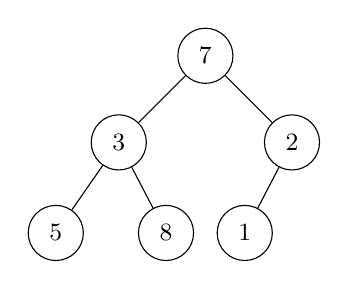
\begin{tikzpicture}[v/.style={circle,draw,minimum size=7mm,inner sep=0pt,font=\small}]
\node[v] (a) at (0,0) {7};
\node[v] (b) at (-1.1,-1.1) {3};
\node[v] (c) at (1.1,-1.1) {2};
\node[v] (d) at (-1.9,-2.25) {5};
\node[v] (e) at (-0.5,-2.25) {8};
\node[v] (f) at (0.5,-2.25) {1};
\draw (a)--(b) (a)--(c) (b)--(d) (b)--(e) (c)--(f);
\end{tikzpicture}
\end{center}
\begin{enumerate}[label=(\alph*)]
\item (5 points) Adjust the binary tree above to establish a max heap. Draw the resulting max heap.
\item (5 points) Draw the resulting max heap after inserting 4 into the max heap in (a).
\item (5 points) Draw the resulting max heap after removing 8 from the max heap in (b).
\end{enumerate}
\end{pastexam}

\begin{pastsoln}
答案（依層序寫成陣列 $A[1..n]$，圖在最後）：
(a) $8, 7, 2, 5, 3, 1$；(b) $8, 7, 4, 5, 3, 1, 2$；(c) $7, 5, 4, 2, 3, 1$。

這棵樹是完全二元樹，依層序放進陣列是 $A[1..6] = 7, 3, 2, 5, 8, 1$，$A[i]$ 的子節點是 $A[2i]$、
$A[2i+1]$（資結書第~7.2.1~節）。 「把這棵樹調整成最大堆積」照資結書第~8.2~節由下而上建堆積
（虛擬碼~8.3）：$i$ 從最後一個有子節點的位置 $\lfloor 6/2 \rfloor = 3$ 往回到 $1$，每個位置做一次
下沉（和較大的子節點比，較小就交換，一路往下）。

\textbf{(a)}
\begin{itemize}
\item $i = 3$：$A[3] = 2$，子節點 $A[6] = 1$，$2 \ge 1$，不動。
\item $i = 2$：$A[2] = 3$，子節點 $5$、$8$，較大的是 $8$，交換：$7, 8, 2, 5, 3, 1$。 $3$ 換到
$A[5]$，是葉節點，停。
\item $i = 1$：$A[1] = 7$，子節點 $8$、$2$，和 $8$ 交換：$8, 7, 2, 5, 3, 1$。 $7$ 到了 $A[2]$，
子節點 $5$、$3$ 都比它小，停。
\end{itemize}
結果 $A = 8, 7, 2, 5, 3, 1$。 檢查：$8 \ge 7, 2$；$7 \ge 5, 3$；$2 \ge 1$，是最大堆積。

\textbf{(b)} 插入 $4$：放在下一個空位 $A[7]$（$2$ 的右子節點），往上浮。 父節點 $A[3] = 2 < 4$，
交換；新的父節點 $A[1] = 8 \ge 4$，停。 結果 $8, 7, 4, 5, 3, 1, 2$。

\textbf{(c)} $8$ 是根，刪掉它就是取出最大值：把最後一個 $A[7] = 2$ 搬到根，$n$ 變成 $6$，再往下沉。
\begin{itemize}
\item $2, 7, 4, 5, 3, 1$：$2$ 的子節點 $7$、$4$，和 $7$ 交換，得 $7, 2, 4, 5, 3, 1$。
\item $2$ 在 $A[2]$，子節點 $5$、$3$，和 $5$ 交換，得 $7, 5, 4, 2, 3, 1$。
\item $2$ 在 $A[4]$，沒有子節點（$8 > 6$），停。
\end{itemize}
結果 $7, 5, 4, 2, 3, 1$。

\begin{center}
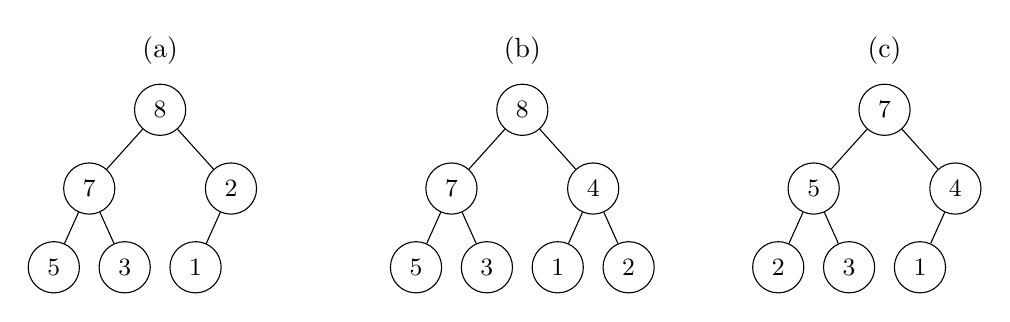
\begin{tikzpicture}[v/.style={circle,draw,minimum size=6.5mm,inner sep=0pt,font=\small},
    level distance=10mm, level 1/.style={sibling distance=18mm}, level 2/.style={sibling distance=9mm}]
\node at (0,0.75) {(a)};
\node[v] at (0,0) {8}
    child {node[v] {7} child {node[v] {5}} child {node[v] {3}}}
    child {node[v] {2} child {node[v] {1}} child[missing]};
\begin{scope}[xshift=4.6cm]
\node at (0,0.75) {(b)};
\node[v] at (0,0) {8}
    child {node[v] {7} child {node[v] {5}} child {node[v] {3}}}
    child {node[v] {4} child {node[v] {1}} child {node[v] {2}}};
\end{scope}
\begin{scope}[xshift=9.2cm]
\node at (0,0.75) {(c)};
\node[v] at (0,0) {7}
    child {node[v] {5} child {node[v] {2}} child {node[v] {3}}}
    child {node[v] {4} child {node[v] {1}} child[missing]};
\end{scope}
\end{tikzpicture}
\end{center}

另一種做法是把 $7, 3, 2, 5, 8, 1$ 依序一個一個插入空的堆積，會得到 $8, 7, 2, 3, 5, 1$，也是最大
堆積，接著 (b)、(c) 分別是 $8, 7, 4, 3, 5, 1, 2$ 和 $7, 5, 4, 3, 2, 1$。 題目說「調整」這棵樹，
指的是原地由下而上建堆積，答案卷上寫第一種，並寫出每一步。
\end{pastsoln}
